
\section{Introduction}
\label{sec:intro}
Software systems are increasingly evolving in their size and complexity.
Large-scale software systems, such as Amazon, Google, and Facebook tend to deal with a high operation workload (e.g., millions of active users), which is complicated by the complexity and the continuous evolution of such systems. Such systems usually report more performance bugs than feature-related ones~\cite{weyuker2000experience}. As such, performance assurance activities are an essential part of the release cycle of such large-scale software systems.

On the other hand, modern large-scale software systems tend to have a large number of configuration options, which can hide performance issues. %For example, Hadoop has over 365 available configuration options~\heng{this is repeated later, may be removed}. 
These options are used to customize the behaviour of a software system without changing its source code. Although these options add flexibility to a software system, they make testing a software performance a challenging task. For example, in theory one has to run $2^
{10}$ tests for a software system with just 10 boolean configuration options, while a highly configurable software system such as \emph{Hadoop} can have as many as 365 available options~\cite{tse}. While there are constraints between configuration options, bringing down the total number of configurations in practice, this still amounts to a too large set of configurations to test exhaustively, especially for (long-running) performance tests.
 
%Therefore, 
A large body of research proposed and evaluated approaches that detect performance issues~\cite{Nguyen:2012:ADP,nguyen2011automated,Nguyen:2014:ICS,foo2010mining,DBLP:conf/icse/FooJAHZF15}. Prior studies also proposed approaches to test the performance of highly configurable software systems~\cite{DBLP:journals/dt/SaxenaFHMYM00,wu2010performance,DBLP:journals/ese/HalinNADPB19}. However, existing approaches aimed at a late stage of the software release cycle, i.e., after the build and deployment of new releases. Nevertheless, identifying performance issues at earlier stages, especially at the development stage, can minimize the amount of resources required for identifying and fixing a performance regression. In fact, going through the whole build, testing, and packaging process to find the root cause of a performance regression is time-consuming. %\bram{is our approach able to achieve this early testing?} \jinfu{Yes, our prediction model can predict whether a CTO manifests performance variation at the commit level.}


% \begin{figure*}[tbh]
% 	\centering
% 		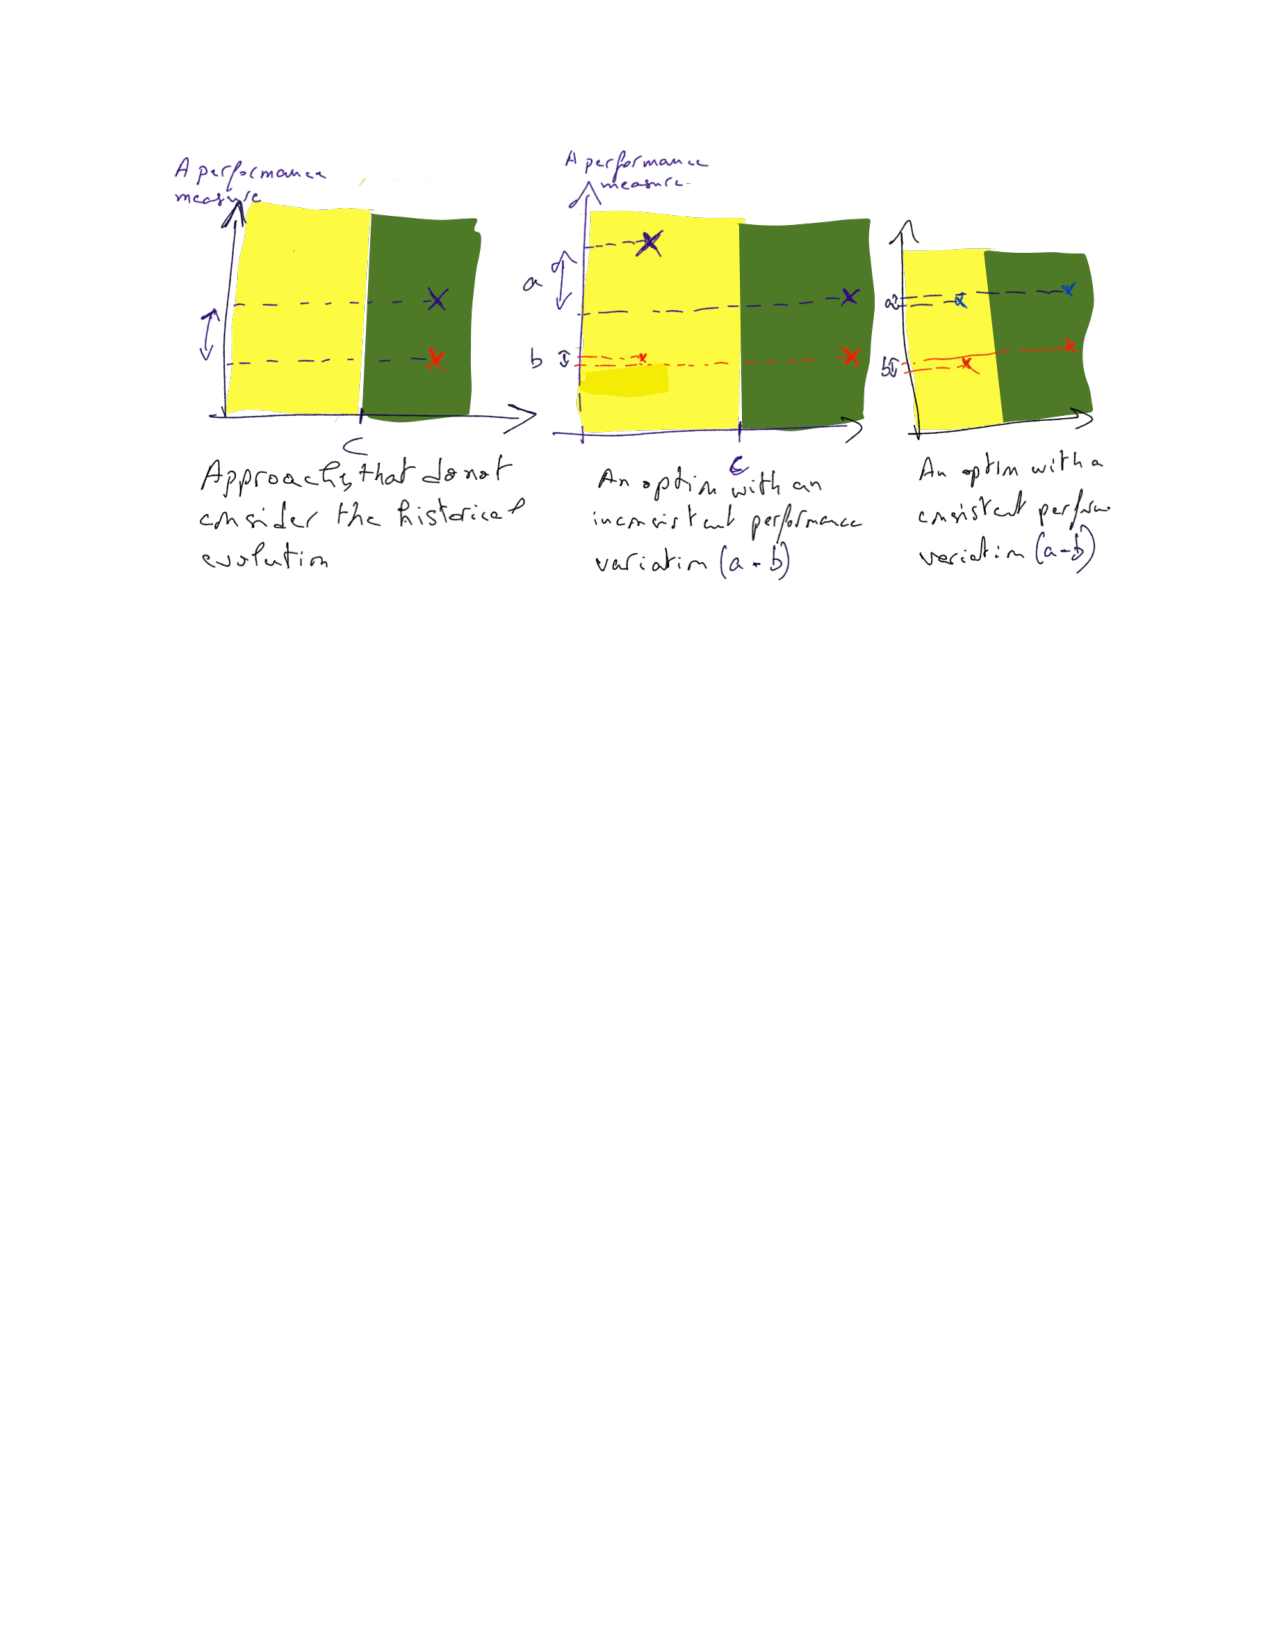
\includegraphics[width=.9\textwidth]{Figures/definition.pdf}
% 		\vspace{-90mm}
% 	\caption{The definition of \inconsistent and how different is it from traditional way of comparing the performance of two values for the same configuration option.\med{todo: label red with v1 and blue with v2}} 
% 	\label{fig:description} 
% \end{figure*}

\begin{figure*}[t]
	\centering
        \begin{subfigure}{0.25\textwidth}
                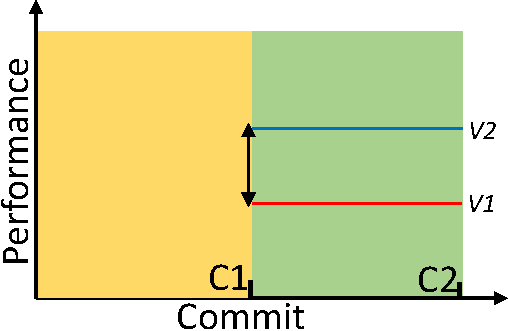
\includegraphics[width=\linewidth]{Figures/background-a.pdf}
                \caption{}
                % \caption{Approaches that donot consider the historical evaluation}
                \label{fig:description-a}
        \end{subfigure}%
        \begin{subfigure}{0.25\textwidth}
                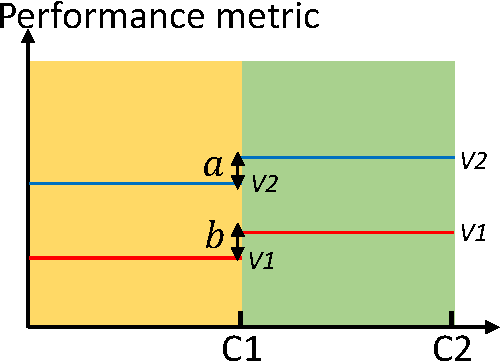
\includegraphics[width=\linewidth]{Figures/background-b.pdf}
                \caption{}
                % \caption{An option with an inconsistent performance variation (a-b).}
                \label{fig:description-b}
        \end{subfigure}%
        \begin{subfigure}{0.25\textwidth}
                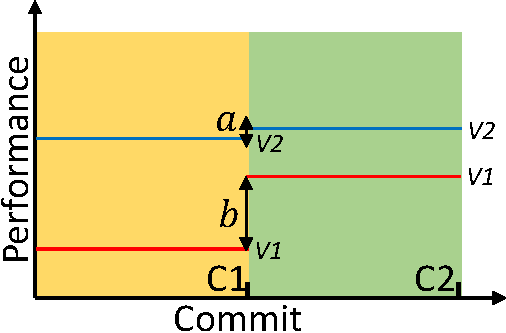
\includegraphics[width=\linewidth]{Figures/background-c.pdf}
                \caption{}
                % \caption{An option with a consistent performance variation (a-b).}
                \label{fig:description-c}
        \end{subfigure}%
        \begin{subfigure}{0.25\textwidth}
                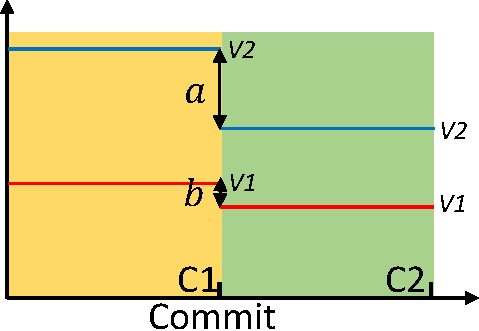
\includegraphics[width=\linewidth]{Figures/background-d.pdf}
                \caption{}
                % \caption{An option with a consistent performance variation (a-b).}
                \label{fig:description-d}
        \end{subfigure}%
	\caption{%\bram{would the figure be easier to interpret if the long blue/red lines also would be just half the length, then put the a/b vertical areas on the border between yellow and green?} \bram{also, would be more logical to first show case c (expected behaviour), then d and b who show variations both for aggravated and improved performance} 
	The definition of \inconsistent and how different it is from the traditional way of comparing the performance of two values for the same configuration option: (a) Approaches that do not consider the historical evaluation, (b) An option with a consistent performance variation (a-b), (c) An option with an inconsistent performance variation (a-b), and (d) An option with an inconsistent performance variation (a-b). V1 and V2 are two different values of the same configuration option. C1 and C2 are two revisions. A smaller performance metric value (e.g., CPU usage) indicates a better performance.
	%\heng{(a) ...; (b) ...; (c) ...; (d).... Then explain what is V1, V2, and what is C1, C2. This is to make the figure self-explainable}. 
	%\heng{Make the longer lines just within the green boxes.} 
	%\heng{A smaller performance metric value (e.g., cpu usage) indicates a better performance.}} 
	}
	\label{fig:description}
\end{figure*}


%Furthermore, prior studies do not consider the evolution aspect when configuration performance. 

Traditionally, prior work studied the difference in system performance caused by \emph{different} values of the \emph{same} option, without considering how the performance impact of an option evolves due to code changes~\cite{tse}. For instance, traditional approaches compare different values of a configuration option based on their raw performances values~\cite{RN2880,RN3537,RN3543}, as illustrated in Figure~\ref{fig:description-a}. However, such comparison is subjective as
the option's value \emph{V2} with worse performance might not necessarily be problematic, but might, as an example, just enable the execution of some extra features.

Conversely, even if an option's value has a good performance compared to other values, those differences in performance might start to vary % still be significantly different
when comparing to the performance of the same option value in the prior commit. Normally, one would expect to see the situation in Figure~\ref{fig:description-b}, which shows that both option values have a consistent variation in performance, in this case a similar increase (regression) in the performance metric. In reality, one can observe %\bram{any indications for this, or at this point in the paper still a hypothesis?} \jinfu{hypothesis} 
cases such as in the example in Figure~\ref{fig:description-c}, where \emph{V1} still shows better performance compared to \emph{V2} after commit C2, but it faces a significantly larger performance regression compared to the prior commit than \emph{V2}. Similarly, in Figure~\ref{fig:description-d}, the \emph{V2} value still has a worse performance after the new commit, but its performance improved much more significantly compared to the prior commit.

%On the opposite side, an option's value that has a better performance compared to another value of the same option might be facing a large performance regression compared to the prior commit, as shown in the example of Figure~\ref{fig:description-d}. 
Therefore, different values of an option can have an inconsistent variation in terms of performance compared to the prior commit, which % . This happens when one or more values of an option exhibit a significant difference compared to the prior release. 
we refer to as \textbf{Inconsistent Option Performance Variation (a.k.a, \inconsistent)}. The \inconsistent might be problematic as it can hide a performance regression that is manifested under one configuration option value. In practice, all to often developers use the default value of a configuration option. However, the default value of a configuration option may cause a performance regression while other values of option have performance improvement. %\bram{value? the ``hiding'' part is not clear}. 
%Similarly, when a default configuration shows a performance improvement, altering one of the options' value may indicate no performance improvement or even a performance regression.  
Such regressions can unfortunately go as unseen to the production environment. The \inconsistent may directly affect the user experience, increase the resources cost of the system and lead to reputational repercussions. 
%\bram{so, the existing ``raw'' approaches would stop after seeing the improvement for the default value, or after seeing that V2 is still worse than V1, while they would ignore the change in variation => it is not clear here how bad such ignored variations are (the ``hiding'' is not clear)}

%In this paper, we instead normalize the performance by considering the prior commit for a tested version. In particular, we measure how much variance exists for an option value between a current version and its prior one. For example, an option X with a value Y in a new commit has a different performance consumption compared to the same option and value prior to the new commit. Then, we study the differences between these last variance to measure if different values for the same option manifest different performances compared to the prior change, which we refer to as ``Inconsistent Options Performance Variation'' (\inconsistent).

%In our prior work~\cite{DBLP:conf/icsm/ChenS17}, we conducted a first step toward assisting practitioners on identifying performance regression at the development stage. In particular, we repetitively execute the existing functional tests or micro-benchmarks for each commit. We identify performance regressions in each test or micro-benchmark if there exists statistically significant degradation with medium or large effect sizes in any performance metric.

In this paper, we perform a case study on two large-scale open-source software systems: \emph{Hadoop} and \emph{Cassandra}. We first conduct a preliminary study to quantify the prevalence of \inconsistent in practice. We observe that 81\% of the commits have at least one option manifesting an \inconsistent issue. We also observe that manually identifying such issues is challenging, as commits do not share the same options that manifest an \inconsistent. That motivates us to propose an automated model that predicts if the combination of a Commit, a Test, and an Option (\textbf{\instance}) would exhibit an \inconsistent issue. We evaluate our explanatory model using the following two research questions: 

%Then, we propose a model to predict which Commit, Test, and Configuration (\textbf{\instance}) might suffer from an \inconsistent, which can be harmful. %the impact of software configuration on hiding performance regression and proposed a prediction model to identify such regressions at the development stage. In fact, software configuration makes the identification of performance regression more challenging. 
 %Therefore, we first quantify how often an \inconsistent can occur. Secondly, we propose and evaluate a prediction model that identifies whether a commit has a performance regression that is hidden under a certain configurations. %In particular, a source code change might not always show a regression, but just under certain configurations. Therefore, in this paper, we quantify the impact of software configurations on hiding performance regression. We then propose a prediction model that combines changed source code as well as configuration related metrics to predict whether a commit has a performance regression that might be hidden by a certain configurations. 
%We summarize our contribution in the following three research questions: 

\begin{itemize}
    
    \item \textbf{RQ1. \RQII}
    
    Our explanatory model reaches an AUC up to 0.93 and 0.90 for predicting \inconsistent for \emph{Hadoop} and \emph{Cassandra}, respectively. We observe that random forest is the most performing model for four and three out of five performance measures (i.e., response time, CPU, memory, I/O Read, and I/O write) for \emph{Cassandra} and \emph{Hadoop}, respectively. 
    
    \item\textbf{RQ2. \RQIII}
    
    We observe that all four dimensions of metrics considered in our study, namely the code structure, code change, code token, and configuration options metrics, have a statistically significant impact in predicting \inconsistent. The dimensions that are related to the configuration options and the tokens of the changed code are the most important dimensions for both case studies. 
    
\end{itemize}

\noindent{Paper organization.} The rest of our paper is organized as follows: Section~\ref{sec:back} provides the background information and defines \inconsistent. Section~\ref{sec:relatedwork} provides prior work related to our paper. Section~\ref{sec:datacollection} discusses our approach of conducting experiments and collecting data. Sections~\ref{sec:pq-results} and~\ref{sec:rq-results} present our results. Section~\ref{sec:threats} discusses the threats to the validity o four findings. Finally, Section~\ref{sec:conclusion} concludes the paper.


%%% Local Variables:
%%% mode: latex
%%% TeX-master: "../main"
%%% End:
